
%%%%%%%%%%%%%%%%%%%%%%% file typeinst.tex %%%%%%%%%%%%%%%%%%%%%%%%%
%
% This is the LaTeX source for the instructions to authors using
% the LaTeX document class 'llncs.cls' for contributions to
% the Lecture Notes in Computer Sciences series.
% http://www.springer.com/lncs       Springer Heidelberg 2006/05/04
%
% It may be used as a template for your own input - copy it
% to a new file with a new name and use it as the basis
% for your article.
%
% NB: the document class 'llncs' has its own and detailed documentation, see
% ftp://ftp.springer.de/data/pubftp/pub/tex/latex/llncs/latex2e/llncsdoc.pdf
%
%%%%%%%%%%%%%%%%%%%%%%%%%%%%%%%%%%%%%%%%%%%%%%%%%%%%%%%%%%%%%%%%%%%


\documentclass[a4paper]{llncs}

\usepackage{amssymb}
\setcounter{tocdepth}{3}
\usepackage{graphicx}
\usepackage[spanish]{babel}

\usepackage{float}
\usepackage{booktabs}
\usepackage{tabularx}
\usepackage{array}
\usepackage{subcaption}
\usepackage{hyperref}


\usepackage{url}
\urldef{\mailsa}\path|nicomad@frba.utn.edu.ar|
\urldef{\mailsb}\path|cad@uns.edu.ar|
\urldef{\mailsc}\path|apousa@lidi.info.unlp.edu.ar|    
\newcommand{\keywords}[1]{\par\addvspace\baselineskip
\noindent\keywordname\enspace\ignorespaces#1}

\begin{document}

\mainmatter  % start of an individual contribution

% first the title is needed
\title{Influencia del tipo de imagen y la autosimilitud en el rendimiento de la compresión fractal}

% a short form should be given in case it is too long for the running head
\titlerunning{Influencia del tipo de imagen y la autosimilitud en la compresión fractal}

% the name(s) of the author(s) follow(s) next
%
% NB: Chinese authors should write their first names(s) in front of
% their surnames. This ensures that the names appear correctly in
% the running heads and the author index.
%
\author{Nicolás Madeo%
\and Claudio Delrieux\and Adrian Pousa}
%

% (feature abused for this document to repeat the title also on left hand pages)

% the affiliations are given next; don't give your e-mail address
% unless you accept that it will be published
\institute{UNLP\\
\mailsa\\
\mailsb\\
\mailsc\\
}

%
% NB: a more complex sample for affiliations and the mapping to the
% corresponding authors can be found in the file "llncs.dem"
% (search for the string "\mainmatter" where a contribution starts).
% "llncs.dem" accompanies the document class "llncs.cls".
%
\maketitle

\begin{abstract}
La compresión fractal representa una imagen mediante un sistema de funciones iteradas (IFS) basado en la autosimilitud entre bloques rango y dominio. Su rendimiento depende del contenido y la codificación es mucho más costosa que la decodificación.En este trabajo se evalúa la influencia del tipo de imagen y de su autosimilitud percibida sobre la calidad (PSNR, MSE, MAE), la tasa (bpp y relación de compresión) y los tiempos de codificación/decodificación, comparando tres geometrías de bloques con JPEG y PNG. La autosimilitud permite reconstruir mejor las imagenes y el contenido tipográfico es el caso más desfavorable. La tasa queda dominada por la geometría y el formato textual del codebook. JPEG supera al método fractal en tasa-distorsión y tiempo de codificación. PNG refleja la redundancia local, no necesariamente la autosemejanza geométrica.
\keywords{compresión fractal, IFS, autosimilitud, JPEG, PNG}
\end{abstract}


\section{Introducción}

Para representar una imagen digital de forma simple, es suficiente con almacenar cada uno de los píxeles, de forma ordenada, junto con el valor de color o intensidad de cada uno. Esto, si bien es fácil de interpretar, trae consigo un alto costo de almacenamiento. Hoy en día, con el alto volumen de datos manejados a través de dispositivos e Internet, es de suma importancia reducir los costos de almacenamiento y utilizar eficientemente el ancho de banda durante la transmisión. La compresión de datos, en este caso imágenes, busca resolver este problema. Aumentar la eficiencia de almacenamiento y el uso del ancho de banda trae consigo beneficios económicos, así cómo una reducción en los tiempos de transmisión.
    
\subsection{Métodos de compresión}

Un método de compresión transforma una imagen original en una representación digital que requiere una menor cantidad de datos. Existen diversos métodos que aprovechan la redundancia de la información para reducir este tamaño.

Dentro de los métodos de compresión podemos separarlos en dos categorías principales, \textbf{métodos con pérdida} y \textbf{métodos sin pérdida}. La diferencia radica en que los métodos con pérdida priorizan perder algunas partes del conjunto de datos original con tal de representarlo en un tamaño menor, pero manteniendo una calidad aceptable. En cambio, los métodos sin pérdida buscan representar el conjunto de datos original tal cómo se encontraba antes de ser comprimido.

En este análisis vamos a estar enfocándonos en compresión de imágenes y algunos de sus métodos. Un ejemplo de compresión con pérdida es el formato JPEG \cite{wallace1991}, mientras que un ejemplo de compresión sin pérdida es el formato PNG \cite{png2003}.

\subsection{Compresión fractal}
La compresión fractal es un \textbf{método con pérdida} el cual representa a una imagen mediante un conjunto de transformaciones. Estas transformaciones conforman un sistema de funciones iteradas (IFS), que durante la decodificación se aplican repetidamente hasta alcanzar una representación cercana a la imagen original. La representación de estructuras complejas mediante sistemas de funciones iteradas fue desarrollada por Barnsley \cite{barnsley1988}.

Es importante mencionar que la decodificación no requiere una imagen inicial particular, ya que puede comenzar a partir de cualquier imagen o incluso de ruido.

Para entender este método, es necesario entender de dónde provienen estas transformaciones. Estas transformaciones se obtienen a partir de la autosimilitud entre distintas regiones de la imagen original.

Esto es eficaz en gran medida para aquellas imágenes cuyas regiones son similares a otras. Es decir, aquellas imágenes que contengan regiones de sí mismas, que puedan representarse por otras regiones de la misma imagen, podrán reducir su tamaño.

Sin embargo, existe una asimetría entre la codificación y decodificación de las imágenes con compresión fractal. Esto se debe a que obtener el conjunto de transformaciones requiere un gran costo computacional debido a la búsqueda de regiones autosimilares dentro de la imagen.

\subsection{Problema de investigación}

Dado que la autosimilitud puede influir en la eficiencia del método, se identifica la necesidad de entender cómo el contenido de cada imagen influye en el rendimiento de la compresión fractal. ¿Cómo influyen el tipo de imagen y su grado de autosimilitud en la calidad de reconstrucción, la relación de compresión y los tiempos de codificación y decodificación de la compresión fractal en bloques?

\subsection{Objetivo del trabajo}

El objetivo de este trabajo es evaluar la influencia del tipo de imagen y de su grado de autosimilitud sobre el rendimiento de la compresión fractal en bloques. Para ello, se analizarán la calidad de reconstrucción mediante las métricas PSNR, MSE y MAE, la relación de compresión y los tiempos de codificación y decodificación. Los resultados obtenidos se compararán con los correspondientes a los métodos JPEG y PNG.



\section{Antecedentes}

\subsection{Sistemas de funciones iteradas}

Un IFS, o sistema de funciones iteradas, es un conjunto de transformaciones que, aplicadas iterativamente, permiten representar una imagen digital. Estas transformaciones son contractivas, es decir, permiten definir lo que se denomina un atractor. Al aplicar reiteradamente el conjunto de transformaciones sobre el resultado de la iteración anterior, las imágenes obtenidas convergen hacia ese atractor final.

Con esto, se puede alcanzar la representación final de una imagen a partir de la aplicación de un conjunto de transformaciones con distintos parámetros. Barnsley propuso un método que, a partir de un conjunto reducido de transformaciones, permitía representar imágenes complejas utilizando pocos parámetros. Si bien esto fue innovador, presentaba limitaciones para su aplicación sobre imágenes reales, debido a la dificultad de encontrar las transformaciones necesarias para representarlas.

\subsection{Compresión fractal en bloques}

La compresión fractal en bloques surge a partir del método desarrollado por Jacquin \cite{jacquin1992}. El método propone dividir la imagen en bloques y comparar regiones similares dentro de la misma imagen. Esta división definió dos tipos de bloques: los bloques rango y los bloques dominio.

Los bloques dominio se obtienen a partir de la imagen original y tienen un tamaño mayor que los bloques rango. A partir de un bloque dominio se aplican transformaciones geométricas y de intensidad para aproximarlo a un bloque rango.

Una vez definidos los bloques dominio, los bloques rango y las transformaciones aplicables, se buscan similitudes entre cada bloque rango y los bloques dominio transformados. Luego se selecciona, para cada bloque rango, el bloque dominio transformado que produce el menor error.

Las transformaciones geométricas pueden incluir reducción espacial, rotaciones y reflexiones. Las transformaciones de intensidad modifican el contraste y la luminancia del bloque. Una vez encontrada la mejor correspondencia, se almacenan los parámetros de la transformación, como la escala de contraste (s) y el desplazamiento de luminancia (o).

En este trabajo se utilizan imágenes PGM en formato ASCII, donde cada píxel se representa mediante un nivel de gris. Para imágenes en color, el procedimiento debería aplicarse considerando los distintos canales de color.

\subsection{Características, limitaciones y dependencia del contenido}

Dentro de las principales características y limitaciones se encuentra el alto costo computacional durante la codificación, ya que se deben buscar regiones similares, aplicar las transformaciones y almacenar sus parámetros. La decodificación es relativamente rápida, dado que la aplicación de las transformaciones durante un número determinado de iteraciones permite alcanzar una calidad visual aceptable.

También debe existir un compromiso entre la calidad, la relación de compresión y el tamaño de los bloques. Los bloques grandes pueden mejorar la relación de compresión, pero perder detalles. Los bloques pequeños pueden representar mejor bordes y texturas, aunque aumentan el tamaño del código y el costo computacional.

El rendimiento también depende del contenido de la imagen. Las imágenes con regiones uniformes o repetitivas facilitan la búsqueda de coincidencias. En cambio, aquellas con numerosos bordes o texturas, como las imágenes con texto, suelen requerir bloques más pequeños para conservar la calidad.

% Sección "Materiales y métodos" alineada con la implementación real del
% repositorio. Requiere: graphicx, subcaption, booktabs, hyperref.

\section{Materiales y métodos}

\subsection{Conjunto de imágenes}

Para la evaluación se seleccionaron las imágenes Apollonian Gasket, Lena, Baboon y una imagen de un texto extraído del Arte de la Guerra de Sun Tzu. Las imágenes tienen todas un tamaño de $512\times512$ píxeles y se encuentran en los formatos PGM ASCII (P2)\cite{netpbmPGM}, PNG y JPEG, asegurando que todos los métodos partan exactamente del mismo contenido visual. Se definió utilizar estas dimensiones de modo que puedan aplicar a los tamaños de bloques evaluados.

PGM ASCII (P2) representa imágenes en escala de grises mediante valores de intensidad almacenados sin compresión. Este es el formato de entrada usado por el compresor. Las imágenes del experimento y las referencias PNG/JPEG están disponibles en el repositorio del trabajo detallado en la Sección~\ref{sec:entorno_ejecucion}.

\begin{table}[htbp]
\centering
\begin{tabular}{lcrc}
\toprule
Imagen & Dimensión & Tamaño (bytes) & Autosimilitud \\
\midrule
Apollonian Gasket & $512\times512$ & 1\,048\,134 & Alta \\
Lena & $512\times512$ & 966\,593 & Media \\
Baboon & $512\times512$ & 996\,517 & Baja \\
Sun Tzu & $512\times512$ & 1\,027\,181 & Baja (texto) \\
\bottomrule
\end{tabular}
\caption{Conjunto de imágenes utilizado en la evaluación experimental. El tamaño corresponde al archivo PGM ASCII de entrada.}
\label{tab:conjunto_imagenes}
\end{table}

\begin{figure}[htbp]
    \centering

    \begin{subfigure}[b]{0.23\textwidth}
        \centering
        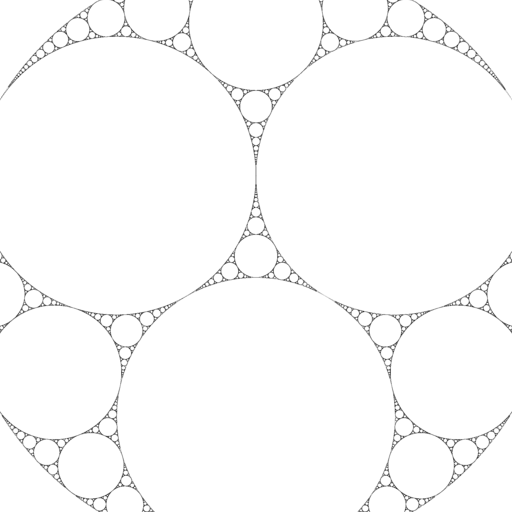
\includegraphics[
            width=\linewidth,
            trim=60 60 60 60,
            clip
        ]{images/apollonian_gasket_512.png}
        \caption{Apollonian Gasket}
    \end{subfigure}
    \hfill
    \begin{subfigure}[b]{0.23\textwidth}
        \centering
        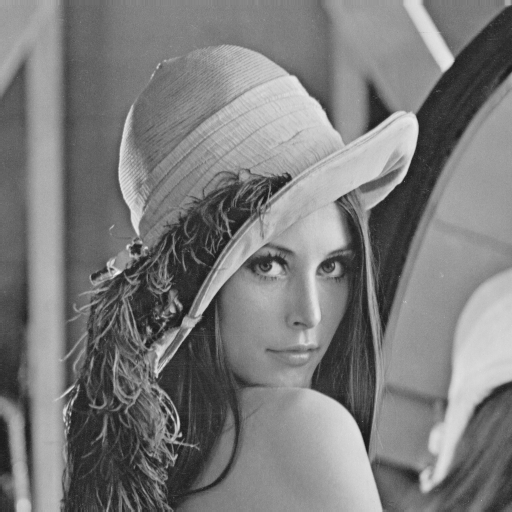
\includegraphics[width=\linewidth]{images/lena.png}
        \caption{Lena}
    \end{subfigure}
    \hfill
    \begin{subfigure}[b]{0.23\textwidth}
        \centering
        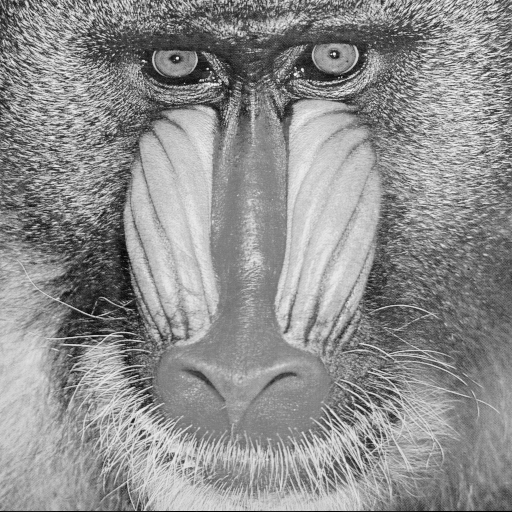
\includegraphics[width=\linewidth]{images/baboon.png}
        \caption{Baboon}
    \end{subfigure}
    \hfill
    \begin{subfigure}[b]{0.23\textwidth}
        \centering
        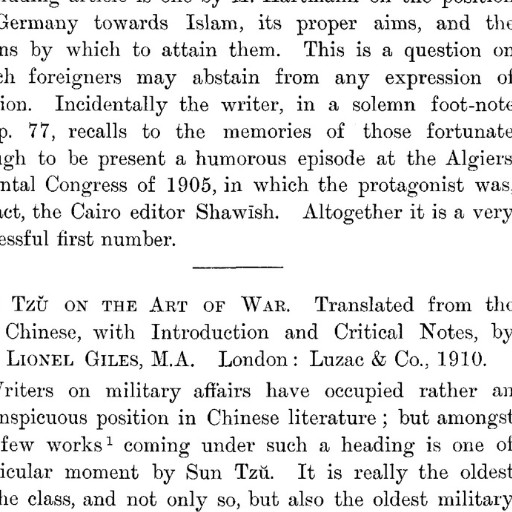
\includegraphics[width=\linewidth]{images/sun_tzu_512.png}
        \caption{Sun Tzu}
    \end{subfigure}

    \caption{Imágenes utilizadas en la evaluación experimental.}
    \label{fig:imagenes_evaluacion}
\end{figure}

\subsection{Clasificación de la autosimilitud}

La autosimilitud fue clasificada de manera perceptiva antes de realizar los experimentos. Para ello, se observaron la presencia de patrones repetitivos, regiones uniformes, texturas y bordes.

\begin{itemize}
    \item Alta: presencia clara de estructuras repetitivas (Apollonian Gasket).
    \item Media: presencia parcial de regiones semejantes (Lena).
    \item Baja: abundancia de texturas, bordes o estructuras poco repetitivas (Baboon).
    \item Baja (texto): predominio de tipografía y bordes agudos sobre fondo uniforme (Sun Tzu).
\end{itemize}

Sun Tzu se incluye como caso de contenido tipográfico, donde la autosimilitud geométrica entre bloques suele ser insuficiente para preservar la legibilidad de los caracteres.

\subsection{Configuración de los métodos}

Para la compresión fractal se utilizaron tres configuraciones:

\begin{itemize}
    \item Bloques rango de $4\times4$ y dominio de $8\times8$.
    \item Bloques rango de $8\times8$ y dominio de $16\times16$.
    \item Bloques rango de $16\times16$ y dominio de $32\times32$.
\end{itemize}

En los tres casos el bloque de dominio duplica el lado del bloque rango, por lo que la reducción al tamaño del rango se realiza con un factor $2{:}1$ mediante el promediado de vecindades de $2\times2$ píxeles. Los bloques rango forman una partición sin solapamiento de la imagen, y los bloques de dominio se toman de una grilla también sin solapamiento.

Se utilizaron ocho transformaciones geométricas básicas: identidad, rotaciones de $90^\circ$, $180^\circ$ y $270^\circ$, reflexiones horizontal y vertical, y reflexiones respecto de las dos diagonales. Para cada bloque rango se evaluaron todos los bloques de dominio reducidos combinados con las ocho transformaciones. Para cada par se calcularon los coeficientes de contraste $s$ y brillo $o$ por mínimos cuadrados, y se conservó la combinación de menor error cuadrático. Para la búsqueda no se aplicó ningún umbral máximo de error ni criterio de terminación anticipada, de modo que el costo de codificación es determinista y depende únicamente de la geometría de bloques.

Cada bloque rango queda descrito por la posición del dominio elegido, el índice de la transformación y el par $(s, o)$. El conjunto de estas asignaciones constituye el \emph{codebook} y es el artefacto que se mide como salida comprimida del método fractal, según se detalla en la Sección~\ref{sec:tamano_comprimido}.

La reconstrucción parte de una imagen inicial de ruido aleatorio y aplica de forma iterativa el sistema de funciones iteradas, lo que permite verificar que el punto fijo alcanzado no depende de la imagen de partida. La calidad se evaluó en las iteraciones 5, 10 y 20. Las iteraciones se indexan desde 0, por lo que las imágenes reportadas como iteración 5, 10 y 20 corresponden, respectivamente, a 6, 11 y 21 aplicaciones del operador de reconstrucción.

Para JPEG se evaluaron niveles de calidad de 25, 50, 75 y 90. Para PNG se utilizó compresión sin pérdida con la configuración predeterminada del codificador. El Cuadro~\ref{tab:referencias} resume los tamaños obtenidos por estas referencias.

\begin{table}[htbp]
\centering
\setlength{\tabcolsep}{10pt}
\begin{tabular}{llrr}
\toprule
Imagen & Formato & Tamaño (bytes) & Bits por píxel \\
\midrule
Apollonian Gasket & PNG     &  23\,039 & 0,70 \\
                  & JPEG 25 &   9\,461 & 0,29 \\
                  & JPEG 50 &  12\,992 & 0,40 \\
                  & JPEG 75 &  17\,487 & 0,53 \\
                  & JPEG 90 &  25\,150 & 0,77 \\
\midrule
Lena              & PNG     & 160\,263 & 4,89 \\
                  & JPEG 25 &  13\,581 & 0,41 \\
                  & JPEG 50 &  20\,913 & 0,64 \\
                  & JPEG 75 &  32\,559 & 0,99 \\
                  & JPEG 90 &  59\,252 & 1,81 \\
\midrule
Baboon            & PNG     & 210\,918 & 6,44 \\
                  & JPEG 25 &  31\,112 & 0,95 \\
                  & JPEG 50 &  48\,852 & 1,49 \\
                  & JPEG 75 &  73\,167 & 2,23 \\
                  & JPEG 90 & 119\,506 & 3,65 \\
\midrule
Sun Tzu           & PNG     & 126\,887 & 3,87 \\
                  & JPEG 25 &  33\,157 & 1,01 \\
                  & JPEG 50 &  48\,442 & 1,48 \\
                  & JPEG 75 &  66\,431 & 2,03 \\
                  & JPEG 90 & 100\,905 & 3,08 \\
\bottomrule
\end{tabular}
\caption{Tamaño y bits por píxel de las referencias PNG y JPEG generadas a partir de los archivos PGM del experimento. PNG es sin pérdida; el número que acompaña a JPEG indica el nivel de calidad.}
\label{tab:referencias}
\end{table}

\subsection{Implementación y entorno de ejecución}
\label{sec:entorno_ejecucion}

La implementación de la compresión fractal fue desarrollada en Java, con codificación y decodificación paralelizadas mediante un pool de hilos de tamaño configurable. Los archivos de referencia PNG y JPEG se generaron con la biblioteca Pillow (que utiliza \textit{libjpeg} y \textit{zlib}) a partir de los mismos archivos PGM empleados por el compresor fractal. El código fuente se encuentra disponible en:

\begin{center}
\url{https://github.com/NicoMadd/fractal-compression/tree/research/paper-autosimilarity-influence-on-fractal-compression}
\end{center}

\begin{itemize}
    \item Procesador: Apple M4 Pro (12 núcleos, arquitectura \texttt{aarch64}).
    \item Memoria RAM: 24\,GiB.
    \item Sistema operativo: macOS 15.1 (build 24B2082).
    \item Versión de Java: OpenJDK 25.0.1, GraalVM CE 25.0.1+8.1 (HotSpot, modo mixto).
    \item Cantidad de hilos: 12 hilos de compresión y 12 de descompresión.
\end{itemize}

Cada configuración se ejecutó una vez por imagen, sin calentamiento previo de la JVM, de modo que los tiempos reportados incluyen el costo de interpretación y de compilación JIT inicial. Por esta razón, los tiempos deben interpretarse como órdenes de magnitud comparativos entre configuraciones y no como mediciones de régimen estacionario.

\subsection{Medición del tamaño comprimido}
\label{sec:tamano_comprimido}

La salida del codificador fractal es un conjunto de asignaciones, una por bloque rango. Cada asignación requiere el índice del bloque de dominio seleccionado, el índice de la transformación aplicada y los coeficientes de contraste $s$ y brillo $o$. Si bien se almacena, la posición del bloque rango no se necesita. Las asignaciones se emiten en el orden de recorrido de la imagen, por lo que el bloque al que corresponde cada una queda determinado de forma implícita por su posición en la secuencia.

El costo de almacenamiento de cada asignación depende de cómo se serialicen esos campos. El archivo \texttt{.fc} que produce la implementación los guarda en representación textual, en la misma línea que el PGM ASCII (P2) de entrada, para que el lector pueda inspeccionar e interpretar el codebook sin herramientas adicionales. Esa decisión prioriza la legibilidad frente a la compactación. Existen formatos binarios o con cuantización de $(s,o)$ que ocuparían mucho menos espacio y harían que las tasas y relaciones de compresión de la prueba fueran sustancialmente distintas a las obtenidas en este trabajo. Los resultados de tasa de este trabajo deben leerse, por tanto, bajo el formato textual adoptado, no como cota del método fractal en general.


\subsection{Métricas y procedimiento experimental}

Se registraron PSNR, MSE, MAE, tamaño original, tamaño comprimido, bits por píxel, relación de compresión y tiempos de codificación y decodificación. Los bits por píxel se calculan como
\[
\mathrm{bpp} = \frac{8 \cdot B}{W \cdot H},
\]
donde $B$ es el tamaño en bytes de la representación comprimida y $W \times H$ la resolución de la imagen.

El PSNR se calcula sobre un rango dinámico de 255 niveles,
\[
\mathrm{PSNR} = 10 \log_{10}\!\left(\frac{255^{2}}{\mathrm{MSE}}\right),
\]
tomando como referencia la imagen PGM original y como estimación la imagen reconstruida en la iteración correspondiente. MSE y MAE se calculan píxel a píxel sobre la totalidad de la imagen.

Para cada imagen se aplicaron las tres configuraciones fractales, los cuatro niveles de JPEG y PNG. Luego se reconstruyeron las imágenes y se compararon la calidad, los tamaños obtenidos y los tiempos de ejecución.

% Sección "Resultados". Requiere: booktabs, float (para [H]).
% Datos generados por data/experiments/run_fractal_experiments.sh,
% measure_reference_metrics.py y summarize_results.py;
% el resumen numérico completo está en data/experiments/results_summary.json.

\section{Resultados}
\label{sec:resultados}

El Cuadro~\ref{tab:comparacion_metodos} reúne las mediciones de tasa, calidad y tiempo obtenidas para las cuatro imágenes bajo las tres geometrías fractales evaluadas y las cinco referencias PNG y JPEG. FBC $r{=}4$ corresponde a la geometría $r=4$, $d=8$; FBC $r{=}8$ a $r=8$, $d=16$; y FBC $r{=}16$ a $r=16$, $d=32$. La relación de compresión se mide respecto de la imagen sin comprimir de un byte por píxel, de modo que los valores menores a $1{:}1$ indican que la salida supera en tamaño a la entrada. El PSNR se reporta en las iteraciones 5, 10 y 20; MSE y MAE corresponden a la iteración 20 (o a la reconstrucción final en PNG y JPEG).

\begin{table}[htbp]
    \centering
    \scriptsize
    \setlength{\tabcolsep}{2.2pt}
    \caption{Resultados de la evaluación experimental. MSE y MAE se reportan en la iteración 20 (FBC) o sobre la reconstrucción final (PNG/JPEG).}
    \label{tab:comparacion_metodos}

    \begin{tabular}{llccccccccrr}
        \toprule
        \textbf{Imagen} &
        \textbf{Método} &
        \textbf{Relación} &
        \textbf{bpp} &
        \multicolumn{3}{c}{\textbf{PSNR (dB)}} &
        \textbf{MSE} &
        \textbf{MAE} &
        \textbf{Cod.} &
        \textbf{Dec.} \\
        \cmidrule(lr){5-7}
        & & & & \textbf{it. 5} & \textbf{it. 10} & \textbf{it. 20} &
        & &
        \textbf{(ms)} & \textbf{(ms)} \\
        \midrule

        Apollonian & FBC $r{=}4$  & $0,62{:}1$  & $12,96$ & $25,74$ & $31,63$ & $32,80$ & $34,12$   & $1,11$  & $14\,450$ & $449$   \\
                   & FBC $r{=}8$  & $2,46{:}1$  & $3,25$  & $24,73$ & $27,11$ & $26,99$ & $129,91$  & $2,91$  & $2\,472$  & $228$   \\
                   & FBC $r{=}16$ & $9,79{:}1$  & $0,82$  & $24,20$ & $24,13$ & $24,17$ & $249,16$  & $4,90$  & $674$     & $236$   \\
                   & PNG          & $11,38{:}1$ & $0,70$  & ---     & ---     & $\infty$ & $0,00$   & $0,00$  & $1,28$    & $0,60$  \\
                   & JPEG 25      & $27,71{:}1$ & $0,29$  & ---     & ---     & $32,40$ & $37,44$   & $1,43$  & $0,25$    & $0,13$  \\
                   & JPEG 50      & $20,18{:}1$ & $0,40$  & ---     & ---     & $35,39$ & $18,82$   & $1,03$  & $0,25$    & $0,14$  \\
                   & JPEG 75      & $14,99{:}1$ & $0,53$  & ---     & ---     & $39,59$ & $7,15$    & $0,65$  & $0,26$    & $0,16$  \\
                   & JPEG 90      & $10,42{:}1$ & $0,77$  & ---     & ---     & $46,68$ & $1,40$    & $0,29$  & $0,28$    & $0,20$  \\
        \midrule

        Lena       & FBC $r{=}4$  & $0,55{:}1$  & $14,57$ & $32,05$ & $35,61$ & $35,64$ & $17,76$   & $2,79$  & $14\,989$ & $440$   \\
                   & FBC $r{=}8$  & $2,20{:}1$  & $3,63$  & $31,04$ & $31,09$ & $31,09$ & $50,57$   & $4,31$  & $2\,626$  & $222$   \\
                   & FBC $r{=}16$ & $8,84{:}1$  & $0,91$  & $26,31$ & $26,48$ & $26,48$ & $146,20$  & $7,24$  & $734$     & $209$   \\
                   & PNG          & $1,64{:}1$  & $4,89$  & ---     & ---     & $\infty$ & $0,00$   & $0,00$  & $3,63$    & $1,60$  \\
                   & JPEG 25      & $19,30{:}1$ & $0,41$  & ---     & ---     & $33,70$ & $27,75$   & $3,74$  & $0,29$    & $0,16$  \\
                   & JPEG 50      & $12,54{:}1$ & $0,64$  & ---     & ---     & $35,81$ & $17,07$   & $2,97$  & $0,31$    & $0,20$  \\
                   & JPEG 75      & $8,05{:}1$  & $0,99$  & ---     & ---     & $37,83$ & $10,71$   & $2,40$  & $0,35$    & $0,27$  \\
                   & JPEG 90      & $4,42{:}1$  & $1,81$  & ---     & ---     & $40,82$ & $5,38$    & $1,75$  & $0,42$    & $0,41$  \\
        \midrule

        Baboon     & FBC $r{=}4$  & $0,54{:}1$  & $14,76$ & $26,26$ & $27,22$ & $27,22$ & $123,37$  & $7,68$  & $15\,101$ & $394$   \\
                   & FBC $r{=}8$  & $2,16{:}1$  & $3,70$  & $21,41$ & $21,45$ & $21,45$ & $466,18$  & $15,23$ & $2\,744$  & $237$   \\
                   & FBC $r{=}16$ & $8,67{:}1$  & $0,92$  & $19,29$ & $19,35$ & $19,31$ & $762,30$  & $20,06$ & $647$     & $233$   \\
                   & PNG          & $1,24{:}1$  & $6,44$  & ---     & ---     & $\infty$ & $0,00$   & $0,00$  & $3,62$    & $1,51$  \\
                   & JPEG 25      & $8,43{:}1$  & $0,95$  & ---     & ---     & $25,30$ & $191,81$  & $10,14$ & $0,37$    & $0,29$  \\
                   & JPEG 50      & $5,37{:}1$  & $1,49$  & ---     & ---     & $27,75$ & $109,19$  & $7,76$  & $0,40$    & $0,40$  \\
                   & JPEG 75      & $3,58{:}1$  & $2,23$  & ---     & ---     & $30,99$ & $51,73$   & $5,49$  & $0,48$    & $0,52$  \\
                   & JPEG 90      & $2,19{:}1$  & $3,65$  & ---     & ---     & $36,95$ & $13,13$   & $2,84$  & $0,53$    & $0,67$  \\
        \midrule

        Sun Tzu    & FBC $r{=}4$  & $0,57{:}1$  & $13,94$ & $20,92$ & $24,55$ & $24,71$ & $219,92$  & $6,40$  & $14\,966$ & $418$   \\
                   & FBC $r{=}8$  & $2,28{:}1$  & $3,51$  & $16,42$ & $16,98$ & $16,93$ & $1\,318,54$ & $18,42$ & $2\,583$ & $222$ \\
                   & FBC $r{=}16$ & $9,05{:}1$  & $0,88$  & $13,95$ & $13,88$ & $13,87$ & $2\,664,80$ & $31,05$ & $758$   & $228$ \\
                   & PNG          & $2,07{:}1$  & $3,87$  & ---     & ---     & $\infty$ & $0,00$   & $0,00$  & $2,96$    & $1,02$  \\
                   & JPEG 25      & $7,91{:}1$  & $1,01$  & ---     & ---     & $25,47$ & $184,62$  & $6,76$  & $0,33$    & $0,26$  \\
                   & JPEG 50      & $5,41{:}1$  & $1,48$  & ---     & ---     & $28,93$ & $83,10$   & $4,76$  & $0,37$    & $0,35$  \\
                   & JPEG 75      & $3,95{:}1$  & $2,03$  & ---     & ---     & $32,96$ & $32,88$   & $3,04$  & $0,40$    & $0,40$  \\
                   & JPEG 90      & $2,60{:}1$  & $3,08$  & ---     & ---     & $51,75$ & $0,43$    & $0,30$  & $0,48$    & $0,57$  \\

        \bottomrule
    \end{tabular}
\end{table}

\section{Discusión}
\label{sec:discusion}

A medida que aumentan el rango y el dominio del FBC, sube la tasa de compresión y en algunos casos supera a JPEG y PNG. También baja el tiempo de compresión: hay menos bloques y la búsqueda de dominio se acorta. El tiempo de decodificación baja en menor medida. Al agrandar el bloque rango, PSNR, MAE y MSE se ven impactados.

Esa superación de JPEG y PNG es de \emph{relación de compresión} (tamaño), no de calidad a igual tasa. Con rango $16$ el FBC ronda $9{:}1$ y en Lena o Baboon supera a PNG en tamaño. Frente a JPEG, a veces el archivo fractal es más chico, pero el PSNR es marcadamente inferior. En Apollonian Gasket, PNG sigue delante ($11{,}38{:}1$ frente a $\sim 9{,}8{:}1$ del FBC con rango $16$). El codebook textual \texttt{.fc} infla los bits por píxel, así que parte de la ventaja aparente depende del formato y no solo del método.

Al agrandar el rango, la calidad empeora: baja el PSNR y suben MSE y MAE. La codificación cae de forma brusca (del orden de $15$\,s con rango $4$ a menos de $1$\,s con rango $16$). La decodificación solo baja de forma moderada ($\sim 400$\,ms a $\sim 220$\,ms) y se estabiliza. Queda la asimetría típica: codificación costosa frente a decodificación relativamente barata, ambas muy por encima de los milisegundos de JPEG y PNG.

Respecto de la pregunta de investigación: en tiempos la autosimilitud no tiene impacto en las pruebas. Los tiempos dependen, al menos en esta implementación, de la cantidad de bloques.

En tasa y bits por píxel la autosimilitud tampoco tiene impacto. A geometría fija, todas las imágenes generan la misma cantidad de asignaciones en el codebook. El formato textual \texttt{.fc} fija un costo alto por asignación e infla los bits por píxel con independencia del contenido.

En calidad sí hay influencia. Las imágenes de autosimilitud alta o media (Apollonian Gasket y Lena) superaron a las de baja (Baboon y Sun Tzu) en PSNR, MSE y MAE. Lena alcanzó el mejor PSNR. Apollonian, pese a no superarla en PSNR, obtuvo el MAE más bajo: error medio menor, con errores locales grandes en los bordes. Baboon y sobre todo Sun Tzu (texto) fueron los peores.

En síntesis, el tipo de imagen y la autosimilitud percibida condicionan sobre todo la calidad del FBC. No explican de forma relevante la tasa ni los tiempos bajo las geometrías y el formato de codebook usados. Menor autosimilitud útil entre bloques (textura fina o tipografía) implica peor PSNR, MSE y MAE. La geometría de bloques domina la tasa y el tiempo.


\section{Conclusiones}
\label{sec:conclusiones}

En este trabajo se evalúa la influencia del tipo de imagen y de la autosimilitud percibida sobre el rendimiento del FBC. Respecto a la pregunta de investigación, podemos determinar que para los casos evaluados sí se detecta una influencia de la autosimilitud en la calidad obtenida de la imagen. En cambio, la tasa y los tiempos de codificación y decodificación casi no dependen de la autosimilitud bajo las geometrías y el formato de codebook usados. La geometría de bloques, en cambio, tiene impacto sobre el tiempo de codificación, el de decodificación y la tasa de compresión obtenida. Frente a JPEG y PNG, podemos observar que en algunos casos la tasa de compresión del FBC fue más alta, pero a costa de perder calidad. Sin embargo, esos códecs aún presentan un mejor rendimiento en la relación entre tasa y distorsión y en el tiempo de codificación sobre los casos evaluados y frente a la implementación fractal realizada.

Como trabajo futuro se podría investigar otras implementaciones de la compresión fractal con bloques de tamaño variable dentro de cada imagen (hoy el tamaño es fijo por corrida), cambiando el tipo de almacenamiento del codebook y aplicando mejoras de cómputo con unidades gráficas. De este modo se podrían hacer pruebas más contundentes que pongan a prueba los códecs antes comparados.


\begin{thebibliography}{5}

\bibitem{barnsley1988}
Barnsley, M.F.:
Fractals Everywhere.
Academic Press, San Diego (1988).

\bibitem{jacquin1992}
Jacquin, A.E.:
Image coding based on a fractal theory of iterated contractive
image transformations.
IEEE Transactions on Image Processing 1(1), 18--30 (1992).

\bibitem{wallace1991}
Wallace, G.K.:
The JPEG still picture compression standard.
Communications of the ACM 34(4), 30--44 (1991).

\bibitem{png2003}
World Wide Web Consortium:
Portable Network Graphics (PNG) Specification, Second Edition.
W3C Recommendation, ISO/IEC 15948:2003 (2003).

\bibitem{netpbmPGM}
Netpbm:
PGM Format Specification.
\url{https://netpbm.sourceforge.net/doc/pgm.html},
consultado el 27 de julio de 2026.

\end{thebibliography}



\end{document}
